\chapter{Platform}
\label{chp:Platform}
A device has been made to generate, receive and analyse flashes. The complete system architecture can be found in figure \ref{fig:systemOveriew}. Each component and their interfaces will be discussed briefly, followed by a section showing the final build of the platform.

\begin{figure}[h]
	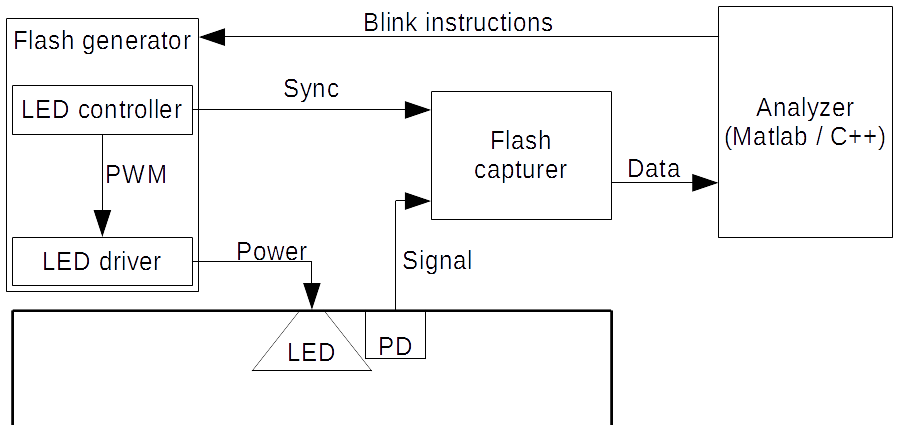
\includegraphics[width=\textwidth]{pics/systemOverview.png}
	\caption{System architecture of the flash generator/analyser}
	\label{fig:systemOveriew}
\end{figure}

\section{system components}

\subsection{Flash generator}
The flash generator is a device able to control a LED with high precision. It is able to set the period $T$, and the t-on time $T_{on}$. $T$ Controls the frequency of the flashes and $t_{on}$ controls the amount of time the LED is turned on. Both parameters can be set with a resolution of $10\mu s$ resulting in a precisely controlled PWM signal. This signal is sent to a LED driver trough one of three LED drivers, which will make the actual light turn on and off at different light levels.

Besides generating the PWM signal for the light, the flash generator has another function. It sends a sync signal to the flash receiver just before generating a flash. This allows the Flash generator to be ready when the flash starts, so it does not waste time sampling if no flash is generated.

\begin{equation}
\label{eq:1/f=T}
T=\frac{1}{f}
\qquad
DutyCycle=\frac{T_{on}}{T} * 100\%
\end{equation}

%\begin{figure}[]
%	\centering
%	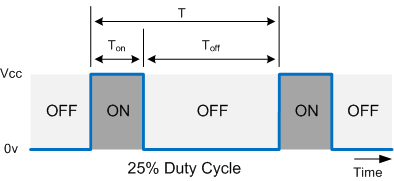
\includegraphics[]{pics/DutyCycle.png}
%	\caption{Visualization of how $T$ and $T_{on}$ determine the duty cycle and frequency of the flash generator}
%	\label{fig:DutyCycle}
%\end{figure}

\subsection{Reflection receiver}
The job of the receiver is to sample values while the light is being turned on and off, to then analyse the full flash and extract it's features. The receiver should start sampling when the sync signal of the flash generator arrives, until the light turns off. Then, the device should do one of the following things, depending on the system settings:
\begin{enumerate}
	\item Send back the full flash, uncompressed, for analysis of separate flashes.
	\item Send back all compressed flashes, by extracting several features.
\end{enumerate}

\subsection{Analyser}
The analyser will receive samples from the reflection receiver and is ran on a PC in the form of either a C/C++ program (real-time) or as a MATLAB script (post-time). If the receiver sends raw flashes to the anlyser it can be used to analyse this flash. This mode is used in section \ref{sec:Flash_characteristics} to analyse single flashes to find the ideal settings for the flash generator and reflection receiver. If the receiver sends compressed flashes, the analyser is able to analyse consecutive flashes. This mode will be used in chapter \ref{sec:Algorithm} to find an algorithm to determine if an object is moving in the area under the light.

The Analyser should also be able to control the flash generator if the system is running in real-time mode. It is therefore able to send a packet with $T$, ${T_on}$ and $LED_{nr}$ to the device. This allows for real time control of the device.

\section{Implementation}
The system was build up with off the shelve parts. pictures of the acutal build can be seen in figure \ref{fig:acutalBuild}. This section will explain briefly how each system component is implemented.

\begin{figure}
	\centering     %%% not \center
	\label{fig:acutalBuild}
	\subfigure[Top view]{\label{fig:top}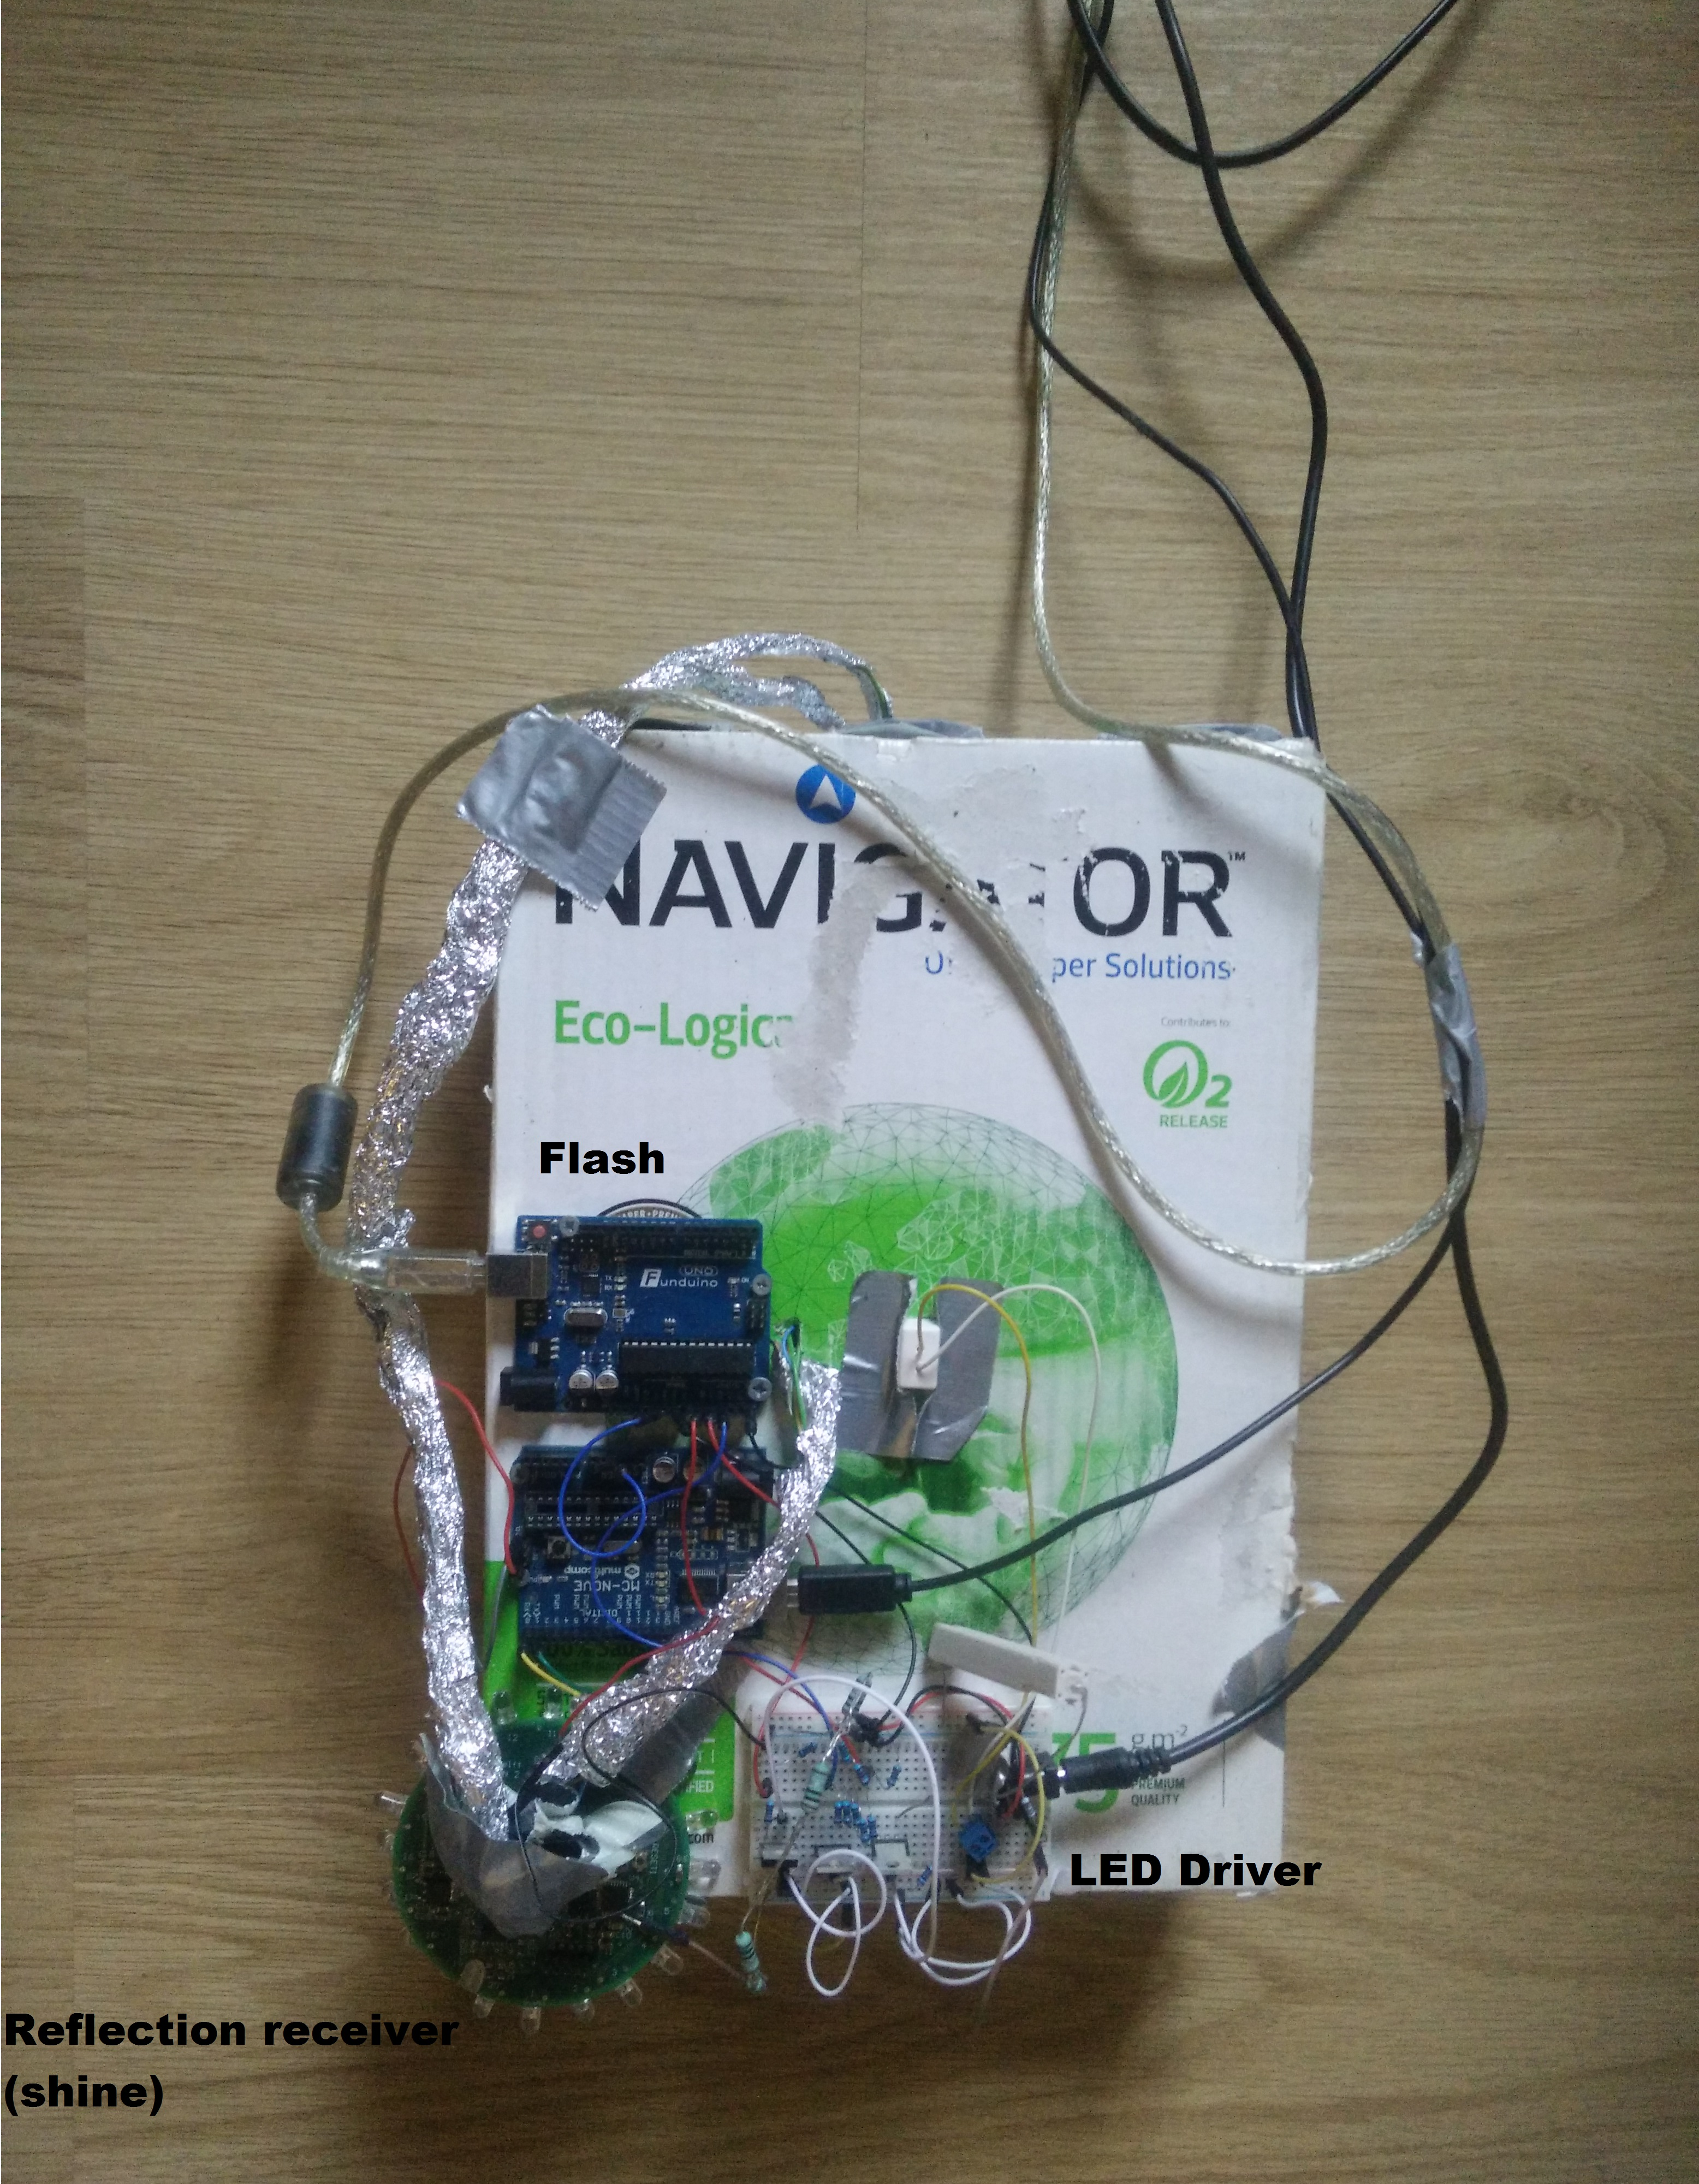
\includegraphics[width=60mm]{pics/platform_top.jpg}}
	\subfigure[Bottom view]{\label{fig:bot}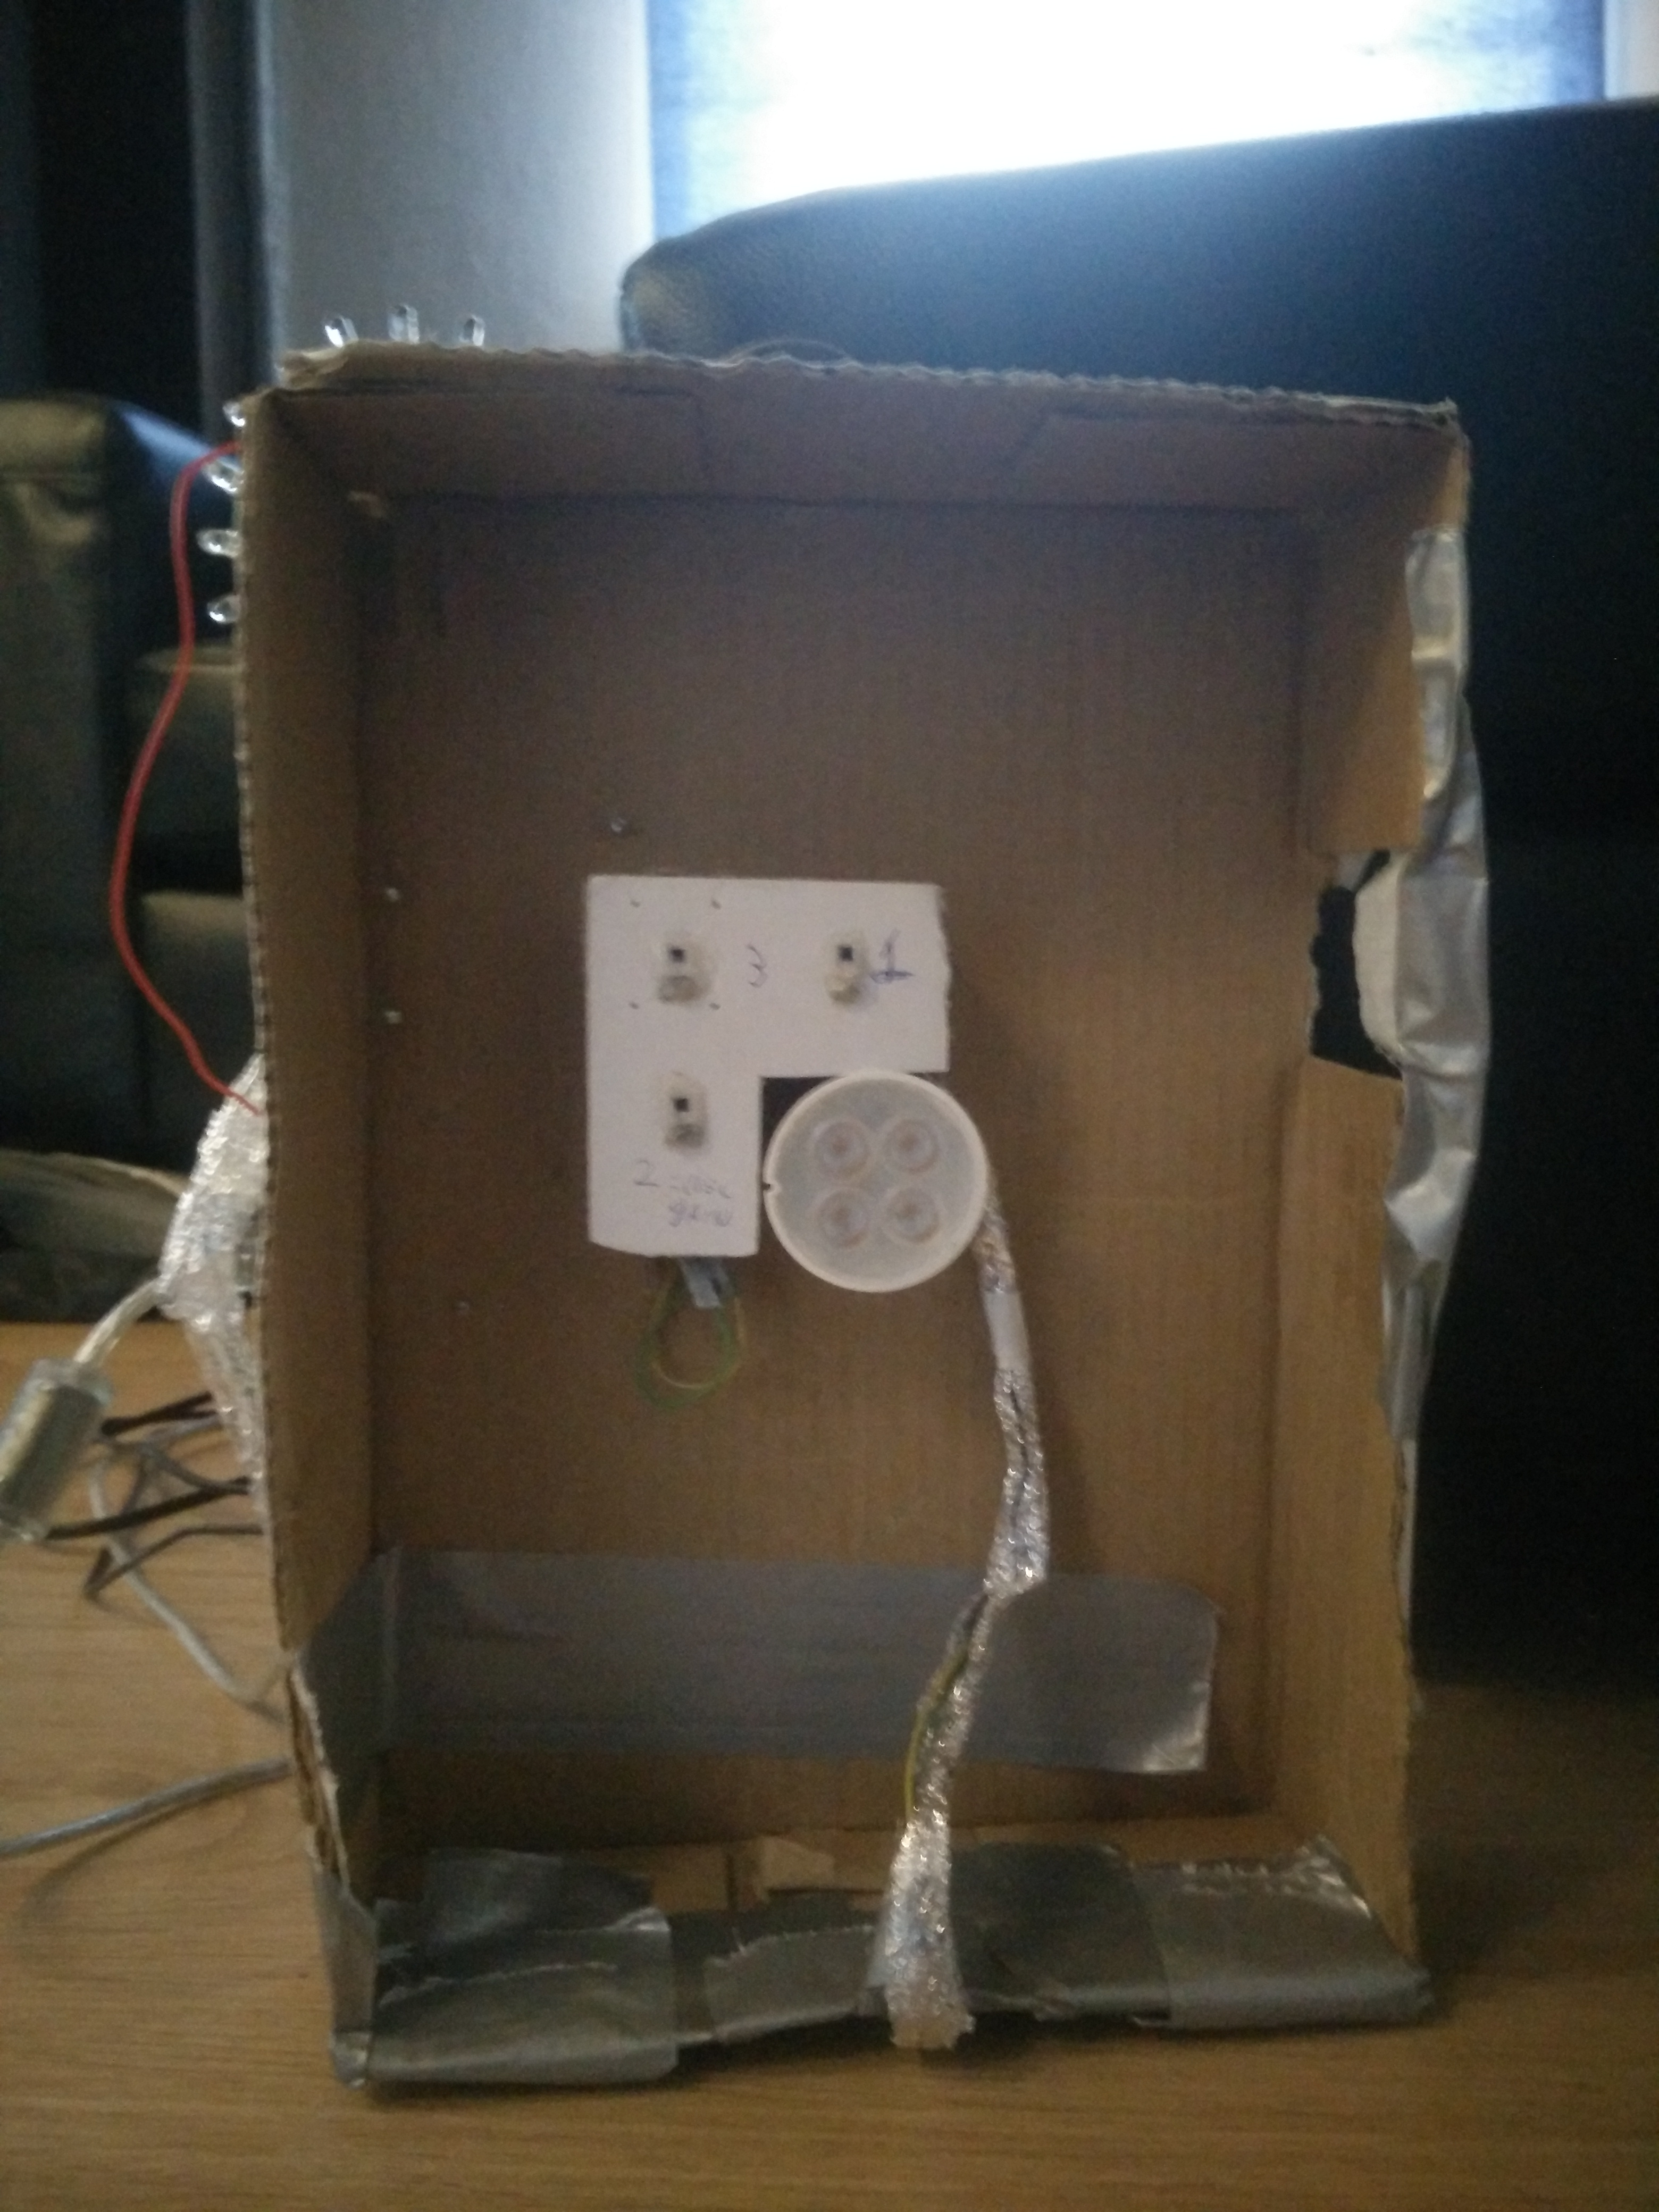
\includegraphics[width=60mm]{pics/platform_bot.jpg}}
	\caption{The used platform in it's bodged glory!}
\end{figure}